
\section{Limit Theorems \skript{43-46}}
\begin{liste}
\item The law of large numbers:
	$\Rightarrow$ Es is prinzipiell möglich, den Erwartungswert einer Zufallsvariablen durch (unendlich) oftes Wiederholen zu bestimmen.\\
	$\lim\limits_{n \rightarrow \infty}{\frac{X_1+X_2+\ldots+X_n}{n}}=\mu$
\item Central limit theorem\\
	$\Rightarrow$ Die Summe einer grossen Zahl von unabhängigen Zufallsvariablen befolgt asymptotisch eine stabile Verteilung $\to$ Normalverteilung.\\
	$\{X_1,X-2,\ldots\}$ is a sequence of independent and identically distributed RV's with $E(X_i)=\mu$ and $Var(X_i)=\sigma^2$. Then the distribution converges to the standard normal as $n\rightarrow\infty$.\\

$\lim\limits_{n \rightarrow \infty}{P\left(\frac{X_1+X_2+\ldots+X_n-n\mu}{\sigma \sqrt{n}}\leq a\right)}=\frac{1}{\sqrt{(2\pi)}}\int\limits_{-\infty}^{a}{\e^{-x^2/2}dx}$
\end{liste}

\newpage

\section{Conditional Probabilities \skript{47-62}}
$\boxed{P_{X|Y}=P(X=x|Y=y)=\frac{P(X=x,Y=y)}{P(Y=y)}}$\\

\begin{tabular}{lll}

  & \textbf{Conditional Cumulative Distribution Fct} & \textbf{Conditional Expectation}\\[0.3cm]
  
Definition & $\boxed{F_{X|Y}(x,y)=P(X \leq x|Y=y)}$ & $E(X|Y=y)$\\[0.3cm]
Continuous & $F_{X|Y}(x,y)=\int\limits_{-\infty}^{x}\frac{f(\tilde{x},y)}{f_Y(y)}d\tilde{x}$	& $E(X|Y=y) = \int\limits_{-\infty}^{\infty}xf_{X|Y}(x|y)dx = \int\limits_{-\infty}^{\infty}x\frac{f(x,y)}{f_Y(y)}dx$\\[0.5cm]
Discrete   & $F_{X|Y}(x,y)=\sum\limits_{x} \frac{P(X=x, Y=y)}{P(Y=y)}$ &	$E(X|Y=y) = \sum\limits_{x} x P(X=x|Y=y) = \sum\limits_{x} x \frac{P(X=x, Y=y)}{P(Y=y)}$\\
\end{tabular}\\

\subsection{A static estimation problem I \skript{56,57}}

One Measurement: $\boxed{Y=X+N}$	
\quad $\boxed{\hat{X}:=f(y)=E(X|Y=y) = y \frac{\sigma_X^2}{\sigma_X^2+\sigma_N^2}}$ 
with error variance $\boxed{\sigma^2=\frac{\sigma_{X}^2 \sigma_{N}^2}{\sigma_{X}^2 + \sigma_{N}^2}}$\\


Theorem: The minimum mean-square error estimator $\hat{X}$ ist the expected value of $X$ knowing the observation $Y=y$.

\subsection{A static estimation problem II \skript{58-60}}

\begin{minipage}{0.6\textwidth}
These are essential ideas behind Kalman filter. Two independent measurements ($z_1, z_2$) at different time.
A model is required: $Z = X + N$ with $Z$ as observation, $X$ the real value and $N$ noise.
	\begin{liste}
	\item Initial condition: Error variance $\sigma_x^2 = \infty$
	\item $t=t_1$:\\
	$\hat{X}(t_1)=\lim\limits_{\sigma_{X}^2 \rightarrow \infty}{E(X(t_1)|Z_1=z_1)}=\lim\limits_{\sigma_{X}^2 \rightarrow \infty}{z_1\frac{\sigma_X^2}{\sigma_X^2+\sigma_{z_1}^2}}=z_1$\\
	$\sigma_x^2(t_1)=\lim\limits_{\sigma_{X}^2 \rightarrow \infty}{\frac{\sigma_X^2 \sigma_{z_1}^2}{\sigma_X^2 + \sigma_{z_1}^2}}=\sigma_{z_1}^2$
	\item $t=t_2$:\\
	
	$\hat{X}(t_2)=\hat{X}(t_1)+K\left(z_2-\hat{X}(t_1)\right)$\\
	$K=\frac{\sigma_{z_1}^2}{\sigma_{z_1}^2 + \sigma_{z_2}^2}$
	with an associated error variance $\sigma^2=\frac{\sigma_{z_1}^2 \sigma_{z_2}^2}{\sigma_{z_1}^2 + \sigma_{z_2}^2}$
	\item Rewritten:\\
	$\hat{z}=\left(\frac{\sigma_{z_2}^2}{\sigma_{z_1}^2 + \sigma_{z_2}^2}\right)z_1 + \left(\frac{\sigma_{z_1}^2}{\sigma_{z_1}^2 + \sigma_{z_2}^2}\right) z_2$\\
	$\frac{1}{\sigma^2}=\frac{1}{\sigma_{z_1}^2} + \frac{1}{\sigma_{z_2}^2}$
	
	\end{liste}
\end{minipage}
\begin{minipage}{0.4\textwidth}
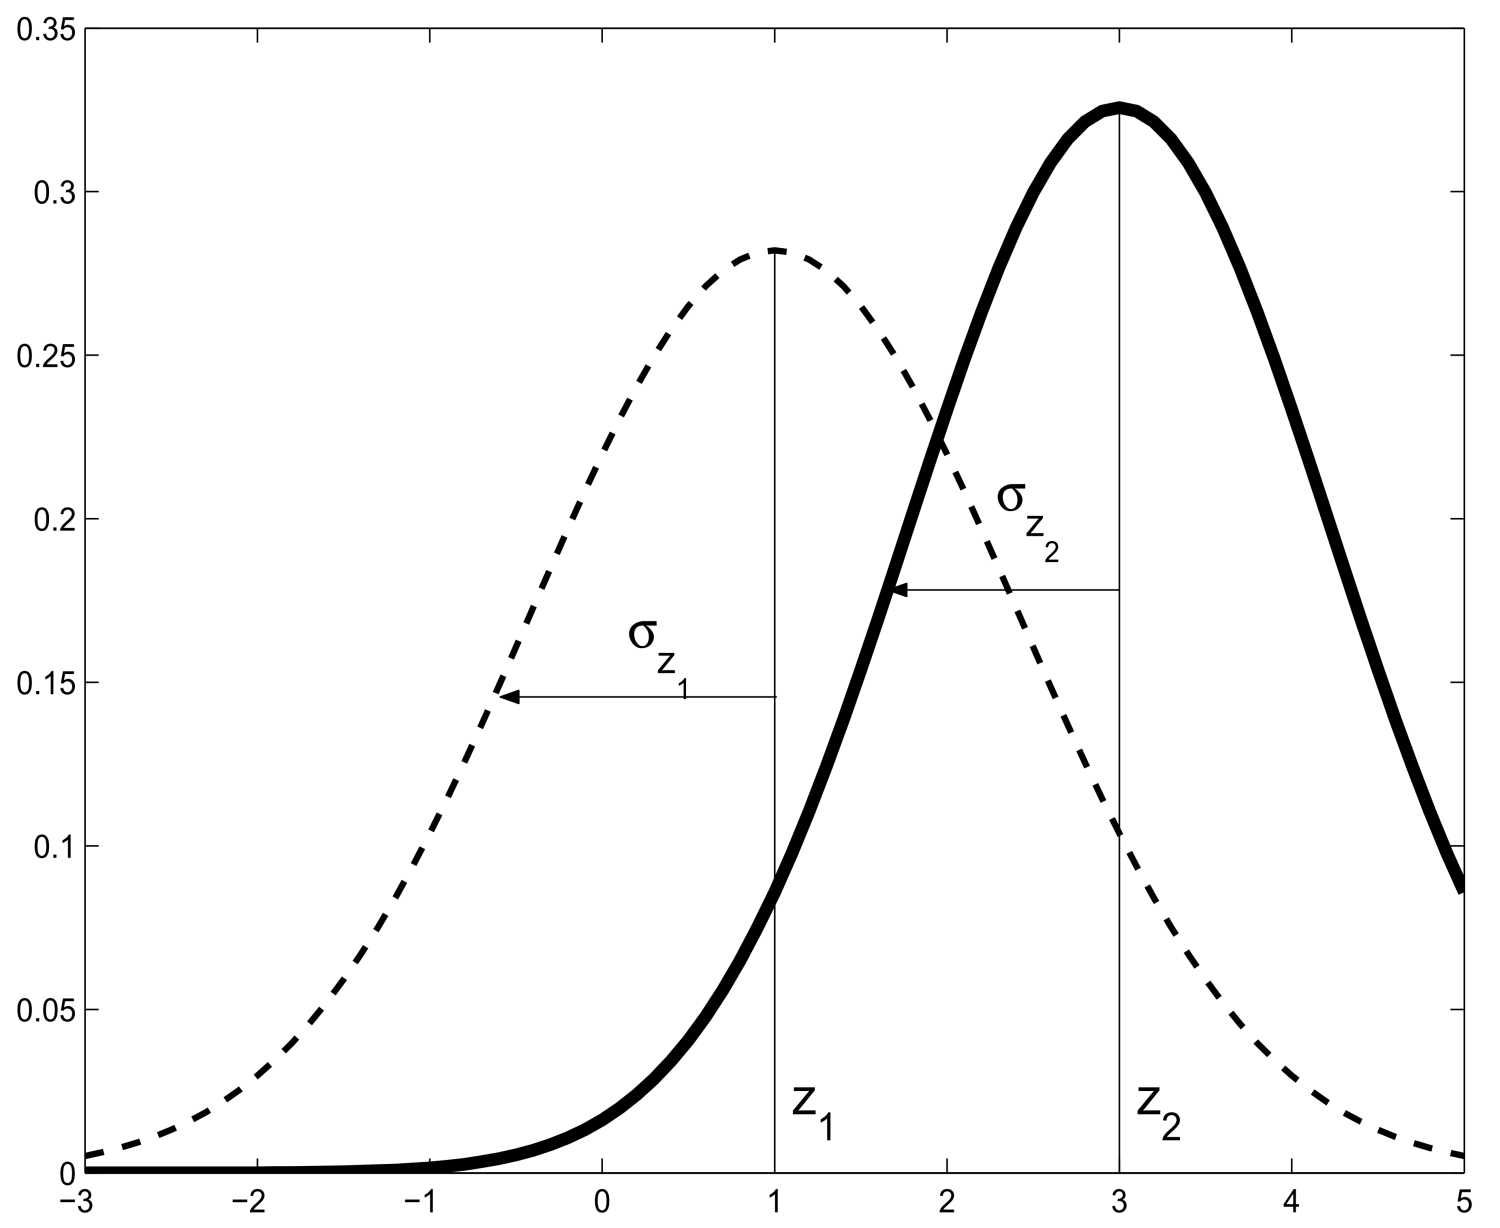
\includegraphics[width=\linewidth]{./Content/LimitTheorems/TwoMeas}
\end{minipage}

\vspace{2mm}
\hrule

